%template for simulation report

\newpage

\section{Cosmos}

\textbf{Object Description:}

\textbf{Simulation Period:} April 2011 
% month and year

\textbf{Science Team contract:} Dave Alexander

\textbf{NuSIM configuration file:}

\textbf{Exposure time:} 6.2 Ms

\textbf{Input Source:} The source list is the 246 objects detected in the 4.5-10 keV band by XMM-Newton. Each object has a SED.

The first row of each file gives the object number, the RA and DEC, and the predicted NuSTAR fluxes in the 6-10 keV, 10-30 keV, and 30-60 keV band (in ergs/s/cm$^{-2}$). The subsequent rows are energy (keV) and flux, where flux is in units of keV$^2$ (Photons cm$^{-2}$ s$^{-1}$ keV$^1$); i.e., what you get from eemodel in XSPEC.

\textbf{Tiling Method:} 122 NuSTAR pointings with half-shift pointing strategy 

\textbf{OA Database Version:} 007
% fill in version number e.g. 008

\textbf{Mast Bend Database:} SAA135
% fill in SAA number

\textbf{Simulation notes:} 
% did we learn anything, did we have to do something special?

\textbf{Status:} 
% are more simulations pending? is it missing something? 

\textbf{Location and name of simulation output:} resource/examples/

\begin{figure}[h]
\begin{center}
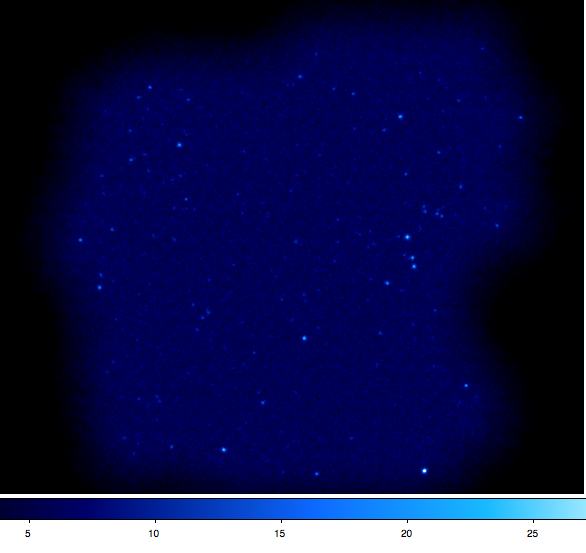
\includegraphics[width=8cm]{Cosmos/cosmos.png}  % if there is an image put it here  
\caption{Cosmos Field. DS9 image. Color scale is linear with lower and upper cuts, and smoothing.}
\label{cosmosimg} 
\end{center}
\end{figure}

\begin{figure}[h]
\begin{center}
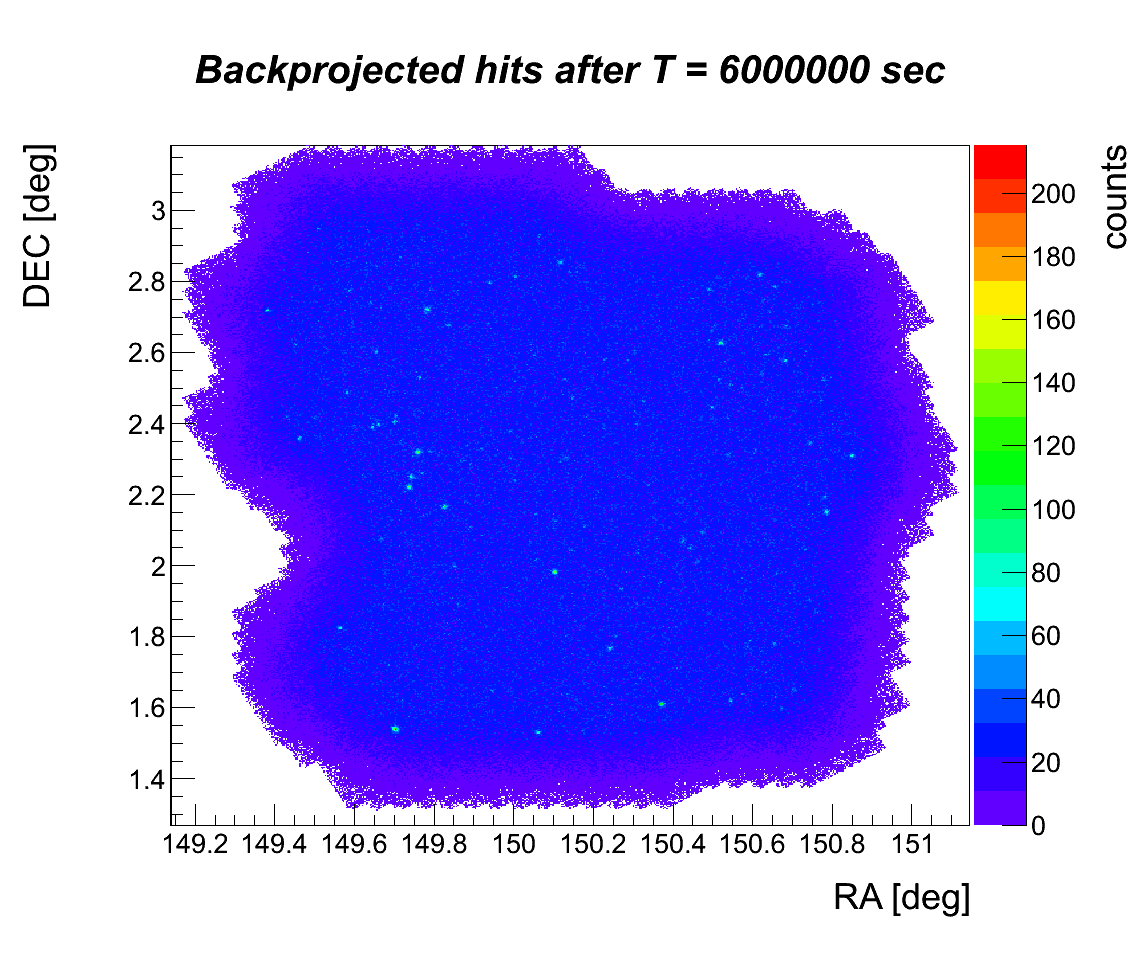
\includegraphics[width=8cm]{Cosmos/Cosmos_v3_noselections.png}  % if there is an image put it here  
\caption{Cosmos Field. NuSIM image.}
\label{cosmosimg} 
\end{center}
\end{figure}

